\section{CIFAR10 example} % Jonathan / b-j8501 / Jul 11 & % b-j8505 / Jul 12
In this section, we will give more details about training a neural network with PyTorch. We will start with the simple CIFAR10 example introduced before, and explain how to modify each component of it. 

The first of all, the first six lines here just consist the \emph{import} statements. Basically all this does is bringing code from this imported libraries from PyTorch in your program allows to use the classes, the functions that for implement each of these libraries.
\begin{python}
import torch 
import torchvision
import torchvision.transforms as transforms
import torch.nn as nn
import torch.nn.functional as F
import torch.optim as optim
\end{python}

\subsection{The \emph{`Net'} class}
Then each neural network we should to implement should exactly contain the class in the following. Which you does is that you define a new class called Net, which is a subclass of nn.Module. The nn.Module is a class implemented in the package torch.nn. Bascially you don't have to know exactly what the Module class does, but the point here is Network is going to be a subclass of it. Let go to it step by step.

Any class defined in Python has to have the \emph{\_\_init\_\_} function. It will run when the class be created. Late on, in the code when you implement like \emph{`conv\_net = Net()'}, it will create an instance of the Net class. And when the instance is created, the \emph{\_\_init\_\_} function is run. And we can see that the \emph{\_\_init\_\_} function create each of the pieces of the neural network, which are the operators we need for our neural network. This linear (\emph{nn.Linear}), convolution (\emph{nn.Conv2d}) and max pool (\emph{nn.MaxPool2d}) is implement in somewhere else. Roughly speaking, they simply contain how much parameters and a forward function. For example the \emph{`nn.Linear'} class: 
\begin{itemize}
\item contains parameters which consists from a matrix and a vector $(W,b)$,
\item and the `forward' function is
$${\rm forward}(x) = Wx+b.$$
\end{itemize}
Later on, we will talk about what \emph{nn.Conv2d} and \emph{nn.MaxPool2d} do.

And then to make is useful, we need to define this forward function. Basically, it tells you, given this neural network and some inputs, what the output is. In this particular case, what the network does is to apply the first convolution, and a ReLU function. The ReLU function is
$${\rm ReLU}(x) = \max\{0,x\}.$$
And then to apply a max pooling. Then applies the next convolution, a ReLU function and pooling layer.
Then, what the \emph{`x.view'} does is take $x$, which is still an image (2 dimensional) and flat it out into a vector. Then applies the first linear layer, a ReLu function, and the second linear layer, a ReLU function, and finally the third linear layer. And it returns $x$. What is contained in the class is all the parameters for each of these layers and the forward function which tells you the order and how to apply them. So that is what network consist.
\begin{python}
class Net(nn.Module):
    def __init__(self):
        super(Net, self).__init__()
        self.conv1 = nn.Conv2d(3, 6, 5)
        self.pool = nn.MaxPool2d(2, 2)
        self.conv2 = nn.Conv2d(6, 16, 5)
        self.fc1 = nn.Linear(16 * 5 * 5, 120)
        self.fc2 = nn.Linear(120, 84)
        self.fc3 = nn.Linear(84, 10)

    def forward(self, x):
        x = self.pool(F.relu(self.conv1(x)))
        x = self.pool(F.relu(self.conv2(x)))
        x = x.view(-1, 16 * 5 * 5)
        x = F.relu(self.fc1(x))
        x = F.relu(self.fc2(x))
        x = self.fc3(x)
        return x
\end{python}

\subsection{The `main' function}
What we want to do is to load a bunch of data, and train this network (all the parameters) on these data. So the \emph{main} function is going to do that. The two lines \emph{trainset} and \emph{trainloader} load the train set, and the two lines \emph{testset} and \emph{testloader} load the test set. The \emph{trainloader} is a class which specifies some way of giving you the data. In our particular case, we construct the \emph{trainloader}, we pass the \emph{trainset}, the images, to it and also a bunch of the parameters, like the batch size, shuffle, number of workers. When you calculate the gradient, you don't use the whole dataset at once, and we only use some of them. The number of data we use to calculate the gradient is the batch size. Here we pass the \emph{`batch\_size'} to the \emph{DataLoader} what happen is the later on when we loop over everything in the \emph{trainloader} (see the for loop in the main function), it will return the images four at a time because we set `batch\_size=4'. The shuffle is true means that you return the data without replacement. It the same thing to the test set.

The \emph{criterion} is a class containing the loss function. Given the output of the neural network and the true label applies the loss function. The optimize class, we will talk about it later on. When you construct the \emph{`optim'} class,  the parameters you have to pass are \emph{`net.parameters'} that tell the optimizer which parameters need to be optimized, and other hyperparameters. It has a function called \emph{`step'}. Whenever the \emph{`step'} function is called it going to modify the parameters in some way based on whatever the gradients are. The optimizer assume you already calculated the gradients and then it does some sort of step based on the gradients. That explains why when you actually run the training we have to call \emph{`optimizer.zero\_grad'} and \emph{` loss.backward'} independently of \emph{`optimizer.step'}. \emph{`optimizer.step'} doesn't handle taking the gradient, it assumes that all the gradients already been taking properly.
 
\begin{python}
def main():
	transform = transforms.Compose([transforms.ToTensor(),transforms.Normalize((0.5, 0.5, 0.5), (0.5, 0.5, 0.5))])
	trainset = torchvision.datasets.CIFAR10(root='./data', train=True,download=True, transform=transform)
	trainloader = torch.utils.data.DataLoader(trainset, batch_size=4, shuffle=True, num_workers=2)
	testset = torchvision.datasets.CIFAR10(root='./data', train=False, download=True, transform=transform)
	testloader = torch.utils.data.DataLoader(testset, batch_size=4, shufflex=False, num_workers=2)

classes = ('plane', 'car', 'bird', 'cat',
           'deer', 'dog', 'frog', 'horse', 'ship', 'truck')
           
conv_net = Net()

criterion = nn.CrossEntropyLoss()
optimizer = optim.SGD(net.parameters(), lr=0.001, momentum=0.9)
 
for epoch in range(2):  # loop over the dataset multiple times

    running_loss = 0.0
    for i, data in enumerate(trainloader, 0):
        # get the inputs; data is a list of [inputs, labels]
        inputs, labels = data

        # zero the parameter gradients
        optimizer.zero_grad()

        # forward + backward + optimize
        outputs = net(inputs)
        loss = criterion(outputs, labels)
        loss.backward()
        optimizer.step()

        # print statistics
        running_loss += loss.item()
        if i % 2000 == 1999:    # print every 2000 mini-batches
            print('[%d, %5d] loss: %.3f' %
                  (epoch + 1, i + 1, running_loss / 2000))
            running_loss = 0.0

print('Finished Training')

correct = 0
total = 0
with torch.no_grad():
    for data in testloader:
        images, labels = data
        outputs = net(images)
        _, predicted = torch.max(outputs.data, 1)
        total += labels.size(0)
        correct += (predicted == labels).sum().item()

print('Accuracy of the network on the 10000 test images: %d %%' % (
    100 * correct / total))

\end{python}

\subsection{\emph{`DataLoader'}}
Next, we want to talk about how can we change the Dataloader and how can we make it provide the data samples in a different way. In particular, we already talk about the difference between sampling with and without replacement. Let us recall that a little bit.

The loss function:
$$L(\theta) = \sum_{i=1}^n l(x_i,\theta)$$
we want to calculate the gradient of the loss function. 
$$\nabla L(\theta) = \sum_{i=1}^n \nabla_\theta l(x_i,\theta)$$
and $n$ generally could be very large, $n \sim 10^4 - 10^7$. In this situation, to compute the gradients over all the data point is computationally not feasible. So just approximate the gradients by sampling some of the data points. 
Initially, consider the computation complexity. Stochastic gradient descent
\begin{itemize}
\item approximate the gradient by considering a sample of data points 
$$\{x_{i_1}, \ldots, x_{i_k}\}$$
where $\{i_1, \ldots, i_k\}$ is randomly chosen in each iteration, then
$$\nabla L(\theta) \approx \sum_{l=1}^k \nabla_\theta l(x_{i_l},\theta)$$
\item $k$ is called the mini-batch size (controls the accuracy of "noise" in the sample).
This is a sampled gradient, containing some noise. If I have larger mini-batch size, we will get a more accuracy gradients, so the mini-batch size $k$ is an important hyper-parameter.
\item $i_1, \ldots, i_k$ sampled with/without replacement.
\begin{itemize}
\item with replacement: there can be repetitions
\item without replacement: there can't be repetitions
\end{itemize}
\end{itemize}
What we implement is sampling without replacement cross the whole epoch. When we randomly choose these data points, we can't choose the same data points again until we around the whole data set. 

Now, let's see how we can change it. First, go to the PyTorch documents page\footnote{\url{https://pytorch.org/docs/stable/data.html}}. Here is an explanation what exactly is this class does, and the important thing for us is what the possible inputs. So when I construct a DataLoader, I need to pass some variables. Whenever we construct a DataLoader, we have to pass it a dataset because there is no default value. In our program, we passed the train set, CIFAR10. You also can pass something else you want to it. And all the other variables here have some default values. There are options here to keep the defaults or to change it to what you want We can see that some of the defaults actually already changed in our program. Instead of the default value 1, we set the batch size as 4, and shuffle as true instead of false. Now, we know how to change the sampling strategies. We probably want to change some of these other inputs. Look here, we can see the description are. In particular, you will see sampler, the default value be none, which defined the strategy. Most likely, if we construct the samlper and pass it to the DataLoader, we can change the with and without replacement strategy.
\begin{figure}[H]
\centering
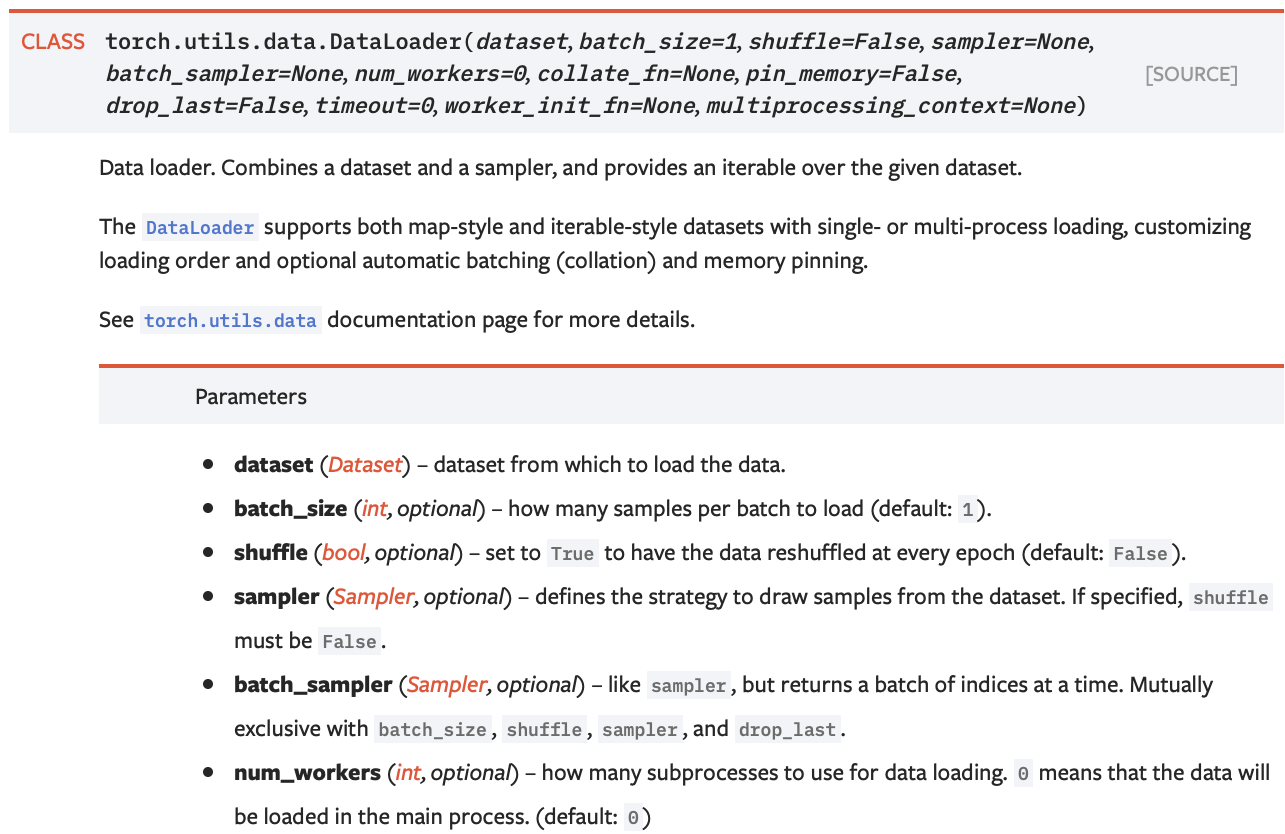
\includegraphics[scale=0.5]{./figures/497Proj_DataLoader}
%\caption{DataLoader}
\end{figure}

Now, we need to look at the sampler class. If we want to change the sampler, we need to define a class that is a subclass of the sampler, and contain the sampler strategy.
\begin{figure}[H]
\centering
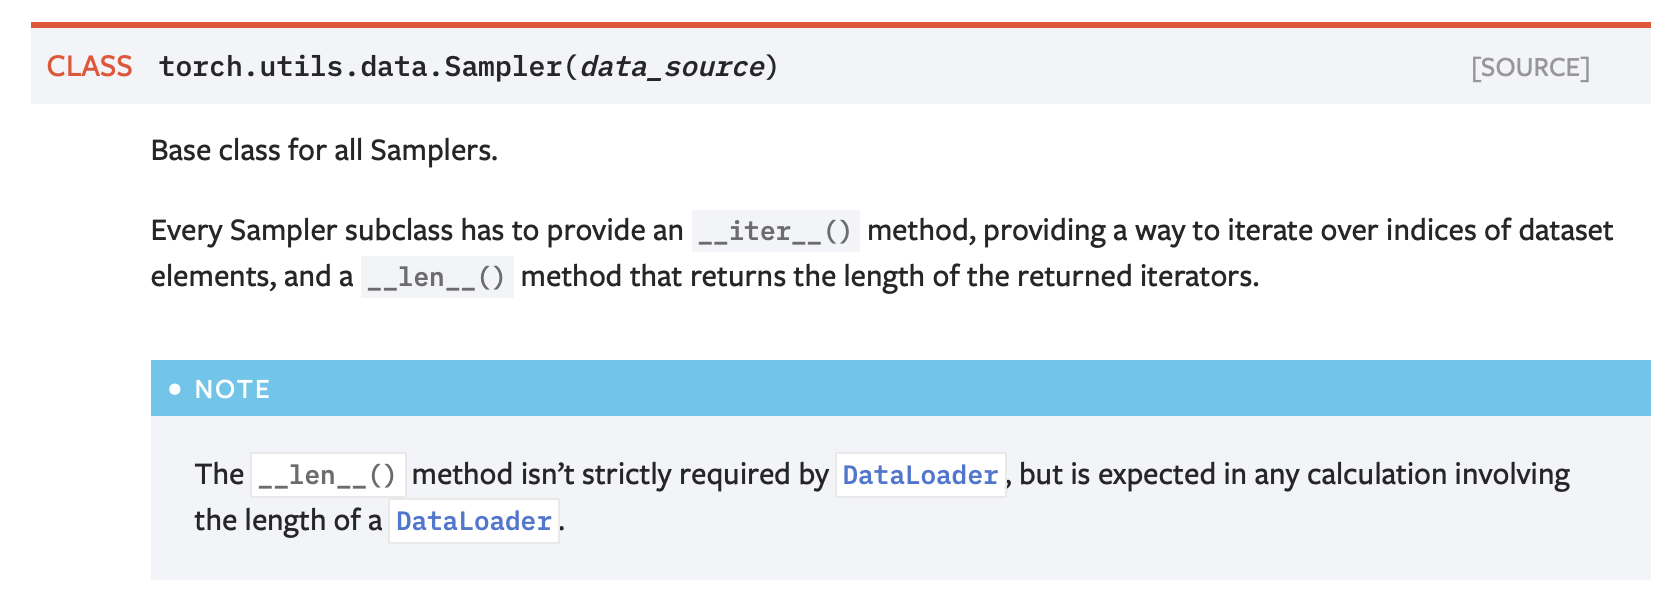
\includegraphics[scale=0.4]{./figures/497Proj_Sampler}
%\caption{}
\end{figure}
In our case, if you want change that with or without replacement, somebody has already written it. 
It turns out the RandomSampler.
\begin{figure}[H]
\centering
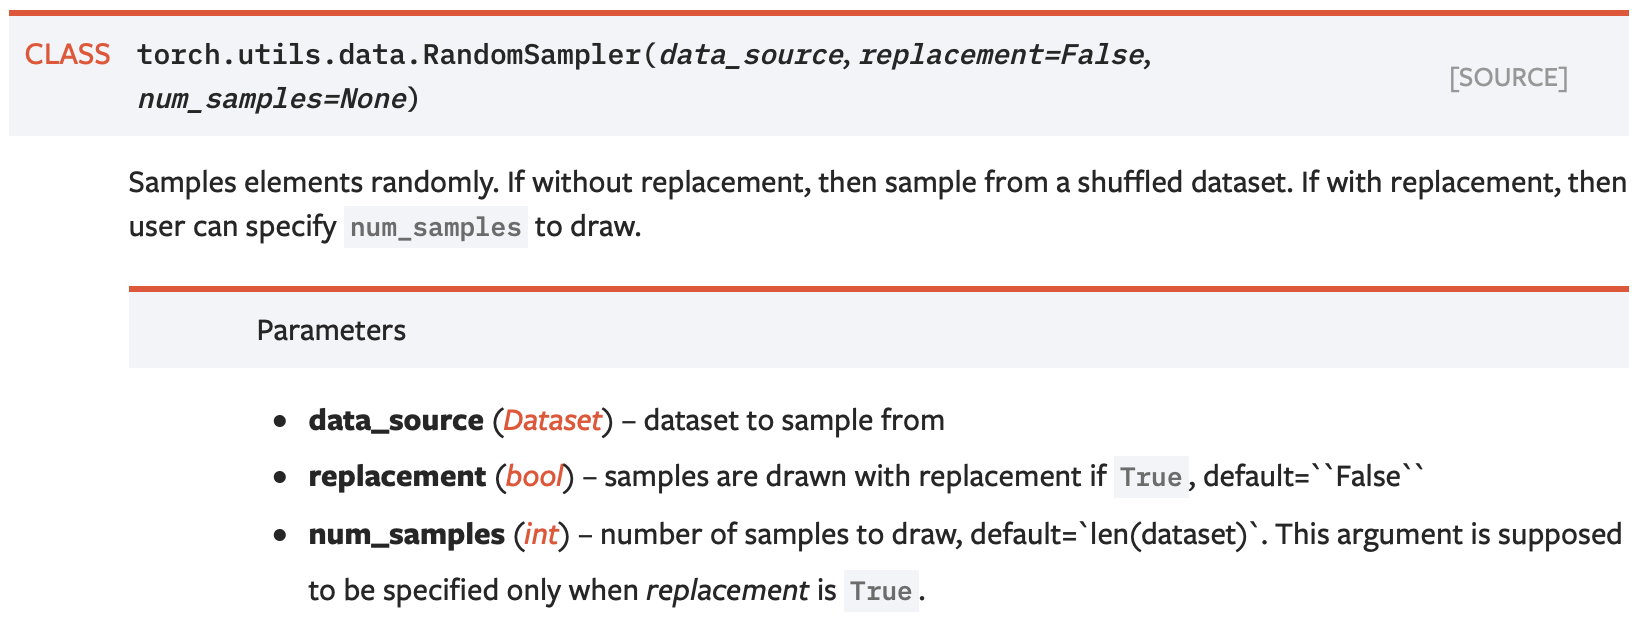
\includegraphics[scale=0.4]{./figures/497Proj_RandomSampler}
%\caption{}
\end{figure}
Let's use our program as an example to show how to use a sampler class. First, we need to create an instance of the RandomSampler class and pass it to the DataLoader as the sampler variable.
\begin{python}
	transform = transforms.Compose([transforms.ToTensor(),transforms.Normalize((0.5, 0.5, 0.5), (0.5, 0.5, 0.5))])
	trainset = torchvision.datasets.CIFAR10(root='./data', train=True,download=True, transform=transform)
	with_replacement_sampler = torch.utils.data.RandomSampler(trainset, replacement=True)
	trainloader = torch.utils.data.DataLoader(trainset, batch_size=4, shuffle=True, sampler=with_replacement_sampler, num_workers=2)
\end{python}
Now if we run this code, the data will be sampled with replacement. This is just to illustrate how you go about changing something about the model and the training process. You just look up the classes, look up in the documentation, see what they do. And often the most of thing that you may want to do, someone already program them in a simple way to do them. You can just turn on like we just doing it. Just notice that you don't have to implement it yourself in this case. You just need to look out these classes do and figure out which tools for use. So we recommend just for fun just try to the CIFAR10 example with and without replacement to see difference. 

\subsubsection{Codes for the CIFAR10 example}
\begin{python}
# cifar10_example.py

import torch 
import torchvision
import torchvision.transforms as transforms
import torch.nn as nn
import torch.nn.functional as F
import torch.optim as optim


class Net(nn.Module):
    def __init__(self):
        super(Net, self).__init__()
        self.conv1 = nn.Conv2d(3, 6, 5)
        self.pool = nn.MaxPool2d(2, 2)
        self.conv2 = nn.Conv2d(6, 16, 5)
        self.fc1 = nn.Linear(16 * 5 * 5, 120)
        self.fc2 = nn.Linear(120, 84)
        self.fc3 = nn.Linear(84, 10)

    def forward(self, x):
        x = self.pool(F.relu(self.conv1(x)))
        x = self.pool(F.relu(self.conv2(x)))
        x = x.view(-1, 16 * 5 * 5)
        x = F.relu(self.fc1(x))
        x = F.relu(self.fc2(x))
        x = self.fc3(x)
        return x

def main():
	transform = transforms.Compose([transforms.ToTensor(),transforms.Normalize((0.5, 0.5, 0.5), (0.5, 0.5, 0.5))])
	trainset = torchvision.datasets.CIFAR10(root='./data', train=True,download=True, transform=transform)
	trainloader = torch.utils.data.DataLoader(trainset, batch_size=4, shuffle=True, num_workers=2)
	testset = torchvision.datasets.CIFAR10(root='./data', train=False, download=True, transform=transform)
	testloader = torch.utils.data.DataLoader(testset, batch_size=4, shuffle=False, num_workers=2)

classes = ('plane', 'car', 'bird', 'cat',
           'deer', 'dog', 'frog', 'horse', 'ship', 'truck')

conv_net = Net()

criterion = nn.CrossEntropyLoss()
optimizer = optim.SGD(net.parameters(), lr=0.001, momentum=0.9)

for epoch in range(2):  # loop over the dataset multiple times

    running_loss = 0.0
    for i, data in enumerate(trainloader, 0):
        # get the inputs; data is a list of [inputs, labels]
        inputs, labels = data

        # zero the parameter gradients
        optimizer.zero_grad()

        # forward + backward + optimize
        outputs = net(inputs)
        loss = criterion(outputs, labels)
        loss.backward()
        optimizer.step()

        # print statistics
        running_loss += loss.item()
        if i % 2000 == 1999:    # print every 2000 mini-batches
            print('[%d, %5d] loss: %.3f' %
                  (epoch + 1, i + 1, running_loss / 2000))
            running_loss = 0.0

print('Finished Training')

correct = 0
total = 0
with torch.no_grad():
    for data in testloader:
        images, labels = data
        outputs = net(images)
        _, predicted = torch.max(outputs.data, 1)
        total += labels.size(0)
        correct += (predicted == labels).sum().item()

print('Accuracy of the network on the 10000 test images: %d %%' % (
    100 * correct / total))

\end{python}


\subsection{The training part of CIFAR10 example}
In this section, we will analysis the training part code in the CIFAR10 example. 
\begin{python}
for epoch in range(2):  # loop over the dataset multiple times

    running_loss = 0.0
    for i, data in enumerate(trainloader, 0):
        # get the inputs; data is a list of [inputs, labels]
        inputs, labels = data

        # zero the parameter gradients
        optimizer.zero_grad()

        # forward + backward + optimize
        outputs = net(inputs)
        loss = criterion(outputs, labels)
        loss.backward()
        optimizer.step()

        # print statistics
        running_loss += loss.item()
        if i % 2000 == 1999:    # print every 2000 mini-batches
            print('[%d, %5d] loss: %.3f' %
                  (epoch + 1, i + 1, running_loss / 2000))
            running_loss = 0.0

print('Finished Training')
\end{python}
In particular, we will see what the \emph{loss.backward} and \emph{optimizer.step} do
\subsubsection{\emph{loss.backward}}
Let's start with the automatically differentiation of PyTorch. This function \emph{loss.backward} hides some pretty complicated code that automatically figure out how to calculate the gradient w.r.t. the output.
Let's start with some simple example.
\begin{python}
import torch
from torch.autograd import Variable
x = Variable(torch.randn(3,3), requires_grad = True)
\end{python}
\emph{Variable} is a fundamental data type in PyTorch, which contains a tensor and some other things, like a flag in our example called \emph{requires\_grad}. So if I set \emph{requires\_grad} is true, it just indicating to PyTorch that in the future whatever \emph{x} is involved in (computational graph), it going to calculate the gradient of x. Also, one of the other things the Variable contains is the gradient value. Which right now should be empty. You can check it by running \emph{x.grad}. 
Now let's see what happen when we use this Variable x in some calculations.
\begin{python}
y = torch.sum(x)
\end{python}
Here, \emph{torch.sum} means all the values of x. Here, we create a new variable y which consists of the sum of the entries of x. And PyTorch allows us to automatically calculate the gradient of the output w.r.t. any inputs. This is an extremely simple example.
\begin{equation}
\begin{split}
x &= \left(\begin{array}{ccc} 
	* &\cdots &* \\
	\vdots &\ddots &\vdots \\
	* &\cdots &*
	\end{array}\right) \\
y &=  \left(\begin{array}{c} 
	1 \\ \vdots \\ 1
	\end{array}\right)^\top
	x\ 
	\left(\begin{array}{c} 
	1 \\ \vdots \\ 1
	\end{array}\right)
	=\sum_{i=1}^3 \sum_{j=1}^3 x_{ij} \\
\frac{{\rm d} y}{{\rm d} x} &= \left(\begin{array}{ccc} 
	1 &1 &1 \\
	1 &1 &1 \\
	1 &1 &1
	\end{array}\right) 
\end{split}
\end{equation}
How to let PyTorch compute this. Simply call 
\begin{python}
torch.autograd.grad(y,x)
\end{python}
This function automatically calculate the derivative of the second augment w.r.t the first. And other way, which is more commonly used, is to call 
\begin{python}
y.backward()
\end{python}
This function will calculate the derivative of y w.r.t everything that depends on the requirements of gradients (see the flag \emph{requires\_grad}). In our case, it will calculate the gradient of y w.r.t. x and store the gradient value in \emph{x,grad}.
These are two common ways that let PyTorch to calculate the gradients. We just give a simple example with one input and one output, but this whole thing works even for much more complicated examples with multiple input variables. And PyTorch can automatically calculate the gradients of these variables.

And there is one important thing to note is now if I call the \emph{y.backwark} again, what happen to the \emph{x.grad}? It will keep the same? or it will be changed? The answer is, unfortunately, it adds the gradient to whatever is already stored in the \emph{x.grad}. So, this explains why we have to zero the gradients of all of the parameters (see \emph{optimizer.zero\_grad}) before we call 
\emph{loss.backward} in our codes.

\subsubsection{\emph{optimizer.step}}
The \emph{loss.backward} step calculates the gradients of all of our parameters and stores in \emph{.grad} fields. Now, let's look at our \emph{optimizer}. This \emph{optimizer} may be a class you want to write yourself if you want to try some new algorithm. It will help to know how it works. 
Notice that the function we are calling here is \emph{optimizer.step}. For example, we set optimizer as SGD. After we calculate the gradients of all of the parameters, then we call this step function, it will add the values of the multiplication of learning rate and negative gradients to current values of the parameters. The \emph{optimizer} class assume that gradients already been calculated and stored in \emph{.grad} fields, and the class just decide what to do with the gradients.

Now, let use Logistic regression as an example.
\begin{python}
# lr_example.py

import torch 
import torchvision
import torchvision.transforms as transforms
import torch.nn as nn
import torch.nn.functional as F
import torch.optim as optim


class LogisticRegression(nn.Module):
    def __init__(self):
        super(LogisticRegression, self).__init__()
        self.linear = nn.Linear(10, 5)

    def forward(self, x):
        return self.linear(x)
\end{python}
We just write a logistic regression class with 10 input features and 5 output features. Then we will use this example to see what a the network class exactly contains.
Run the following codes in python terminal
\begin{python}
import torch
from lr_example import LogisticRegression

net = LogisticRegression()
x = torch.randn(10)
y = net(x)
\end{python}
Here we create an instance of LogisticRegression class, and set x as input and y as output. The variables this class contains is the parameters which is a 10-by-5 matrix and a vector as the bias. And take a vector x as input, and apply the forward step (see \emph{net(x)}, `forward' can be dropped), it will run the forward function to calculate $W x+b$.

There is one thing have to know is that when you call \emph{backward} on something has to be a scalar. It can't be for example a tensor. For example, if I try to call \emph{y.backward}, it will be given an error, because you can only call this for scalar outputs. It won't to calculate a Jacobian matrix of a vector output w.r.t. a vector input. However, if you pass it the derivatives of each of this components, then it can continuous do the \emph{.backward} function. So, for example, if we we want to calculate the derivative of the sum of $y$, we can do it as follows:
\begin{python}
y.backward(torch.ones(5))
\end{python}
If you have a vector that you want to call \emph{.backward} on, you have to pass it a vector with the same size, it gives the gradients of each of the components of that vector w.r.t. the output. Actually, it calculate the Jacobian times the vector. In general, it can't calculate the Jacobian of a non-scalar output, but if you know what you want to multiply the Jacobian with, then you can pass it to \emph{.backward} as well. 

Then we can see the parameter of a network 
\begin{python}
params = list(net.parameters())
\end{python}
Now \emph{params} contains matrix $W$ and vector $b$. Also, we can see the gradient values of them. 
\begin{python}
params[0].grad
params[1].grad
\end{python}

Here we give an explanation about it. For $x\in\mathbb{R}^n$ and $y\in\mathbb{R}^d$, $y$ is some function of $x$.
\begin{equation}
\begin{split}
y &= f(x) \\
\frac{{\rm d} y}{{\rm d} x} &= \left(\begin{array}{ccc} 
	\frac{{\rm d} y_1}{{\rm d} x_1} &\cdots &\frac{{\rm d} y_d}{{\rm d} x_1} \\
	\vdots &\ddots &\vdots \\
	\frac{{\rm d} y_1}{{\rm d} x_n} &\cdots &\frac{{\rm d} y_d}{{\rm d} x_n}
	\end{array}\right)  
\end{split}
\end{equation}
In this case, \emph{y.backward()} will return an error, but we can call \emph{y.backward(v)} for some vector $v\in\mathbb{d}$. Then it will calculate 
\begin{equation}
\frac{{\rm d} y}{{\rm d} x}\cdot v = \left(\begin{array}{ccc} 
	\frac{{\rm d} y_1}{{\rm d} x_1} &\cdots &\frac{{\rm d} y_d}{{\rm d} x_1} \\
	\vdots &\ddots &\vdots \\
	\frac{{\rm d} y_1}{{\rm d} x_n} &\cdots &\frac{{\rm d} y_d}{{\rm d} x_n}
	\end{array}\right)  
	\left(\begin{array}{c} 
	v_1 \\ \vdots \\v_d	
	\end{array}\right)  
= \nabla(y\cdot v)
\end{equation}


This is basically because if you want to compute the whole Jacobian matrix, it requires a lot of time and space and it always not necessary. 

Maybe this will make more sense if I set another variable $z$ as the sum of $y$, 
\begin{python}
net.zero.grad()
y = net(x)
z =torch.sum(y)
\end{python}

In our example, we can see $z$ is a function of $y$ and $z = g(y) = y \cdot v$.
If I take \emph{z.backward}, this is the same computation with the previous did. Because the derivatives of $z$ w.r.t. $y$ is $\frac{{\rm d} z}{{\rm d}y} = (1,1,1,1,1)^\top$. This is what the \emph{.backward} does. It calculate the gradients multiplied by the Jacobian of previous layer to get the previous gradients, and so on.
You can call 
\begin{python}
z.backward()
params[0].grad
params[1].grad
\end{python}
and compare the output with the previous one. 

In practice, we would construct some loss function, and call \emph{backward} on it. Particular, in our cifar10 example, it consists of a bunch of parameters, particular, each of these layers has its parameters, and when you call forward, it performs some complicated calculations. It will build some graph that contains all the dependencies of these calculations. And then, after you apply the network
and apply a loss function to it, you call \emph{loss.backward}, this step gives you all the gradients of the parameters, and then this is a special optimizer class, which takes those stored gradients and use them to perform like a forward step. 
The most important thing to remember are don't forget the \emph{optimizer.zero\_grad} because the \emph{backward} step adds the new calculated gradients to that already stored in the \emph{grad} field. Of course, if you have two loss functions, called \emph{loss1} and \emph{loss2}, you can call 
\begin{python}
loss1.backward()
loss2.backward()
\end{python}
and gradients now is the sum of those two gradients.
